










\section{\textit{Shuǒ wén jiě zì}, Xīn Bù 心部}

\subsection{心}
%1. SW 10B 408: 001; DXB 217 (10B 10a); GL vol 11: 4646b; Duan 501 (10B 23b); TKJ 1438; Ozaki vol. 5 (匏): 994.

\begin{tabular}{ll}
%HG: 

\includegraphics[width=1cm]{Appendices/xin1.png}
({\Large{心}}), & \textit{sim}, \\
%G: 
人心 & (as in) ``the heart of man", \\
%SN1: 
土藏. 在身之中。 & 
\makecell[l]{inner organ that belongs under (the agent) Earth. \\  (which is) in the middle of the torso.}
\\
%GS: 
象形。 & (The graph) symbolises the shape. \\
%SN2: 
博士說以爲火藏。 & \makecell[l]{The Explanations by the Doctors of Learning consider \\
this to be the inner organ belonging to (the Agent) Fire.} \\
%SF:	
凡心之屬皆从心。 & 
\makecell[l]{As a matter of principle, all (graphs) 
 classified \\ under {\Large{心}} 
%{\textit{sim}} ``heart'' 
have {\Large{心}} {\textit{sim}} ``heart'' as semantic constituent.}
\end{tabular}


%G     Xǔ Shèn knew that a wide variety of animals have hearts, and that all these hearts are called xīn 心. We need to explain why he defines the word in terms of the human heart, thus committing the notorious lexicographic mistake of using the definiendum as the main part of the definiens. In so doing Xǔ Shèn would appear to have wrongly narrowed the general meaning of xīn while at the same time failing to give a non-circular explication of the meaning of the word.
%    Xǔ Shèn's gloss focusses on the fact that the primary reference of xīn is linked to the physical human heart as the organ of psychology. It is this human psychology aspect of xīn which is pervasively relevant to the explanations of the graphs in the present section. Animal psychology was alien to Xǔ Shèn's conceptual world: to him psychology was human psychology. The definition of xīn, then, addresses not the question of what the word means and what the graph represents, but it draws attention to the semantic scope of the present section or chapter of Shuōwén. It is predominantly concerned with words related to human psychology rather than animal anatomy.
%    Xǔ Shèn's dictionary must be read as a book, and not merely as a collection of glosses. Sections on the radical themselves are best read as concise introductions to the chapters which they introduce.
%SN1 This line provides cosmological speculation regarding the organ of the heart. It constitutes an encyclopaedic explanation of the things rather than of the meaning of lexical entries.
%    It is typical of Xǔ Shèn's explanations of radicals, as opposed to other characters subsumed under radicals, that he often elaborated their meaning and significance in an encyclopaedic manner.
%Literally, the heart is perhaps also construed as situated near the centre of the torso, sh*n 身.
%But the meaning `person' for sh*n 身 is also relevant here, and especially relevant to the role of xīn 心 as the category under which many psychological terms are organised in Shuōwén. Thus the point suggested, but not explicitly made, is that the heart is construed as the centre of the person. The glosses for the inner organs in Shuōwén are instructive: the lungs fèi 肺 are defined simply as jīn zàng y\% 金藏也 ``inner organ belonging under the agent Metal"; the kidneys shèn 腎 are defined as ``inner organ belonging under the agent Water"; the spleen pí 脾 is defined as ``inner organ belonging under the agent earth'' tǔ zàng y\% 土藏也; and the liver g&n 肝 is defined as ``inner organ belonging under the agent Wood". Thus the glosses place the organs in a cosmological scheme rather than attempting any straightforward anatomical definition. Moreover, the glosses on these organs form a coherent system and are not compiled in an ad hoc way for each organ separately. However there are two `earth' intestines and no `fire' intestines, this surely is the background for the diverging opinion of the Bóshì 博士 ``Doctors of Learning".
%GS Graphological analysis is obligatory for radicals, as it is for other characters. Thus the graphemic elements themselves are not treated as graphological atoms: they may be complex, in which case Xǔ Shèn analyses their composition, or they may be simplex – as in the present instance – in which case graphological specification remains obligatory but is not normally in terms of the liùshū 六書. (It should be noted that only the term xiàng xíng 象形 is currently used in Shuōwén, zh+ shì 指事 has been found only twice throughout the text.)
%    In this line the subject has changed: Xǔ Shèn turns from the description of what the word xīn 心 refers to to an explanation of the type of graph used to write that word. Moreover, he never speaks of xiàng xíng zì 象形字 ``a character involving symbolising a shape'' but prefers the verbal formula xiàng xíng 象形 ``(the graph) symbolises a shape". (It would be an arbitrary conjecture to take the verbal formula as elliptic for the more explicit nominal phrase xiàng xíng zì y\% 象形字也.) Even in his postface, Xǔ Shèn does not speak in our modern way of xiàngxíng zì 象形字 but only of xiàng xíng zh\% 象形者 ``those which symbolise shape'' and for example, huì yì zh\% 會意者
%"those which associate ideas".
%SN2 Xǔ Shèn's explicit reference to the bó shì 博士 and their explanations (shuɨ 說) establishes an unusual polemical mode in which he appears to take exception to a predominant view held by the government-appointed specialists bó shì 博士. Without taking sides on the issue at hand one notes



%that the Labor Ministry Official gɨng cáo 功曹 Xǔ Shèn took it upon himself to disagree in writing on important points with the imperially appointed senior specialists.
%    It is surprising to have to note that Xǔ Shèn does not write as a partisan of the so-called gǔwén or jīnwén tradition, but occasionally feels free to agree with either of them when he sees fit. It remains significant, however, that he does not provide arguments for disagreeing with the school of  his  preference,  the  gǔwén  tradition  (see  Miller  1953:  58-59,  M(  Zɨŋhuò  Shuōwén  ji\%z+  y+n tɨngrén k(o 1967: ch. 3, p. 27).
%The subject of the verb y+ wéi 以為 ``to imagine, to hold to be true'' is never an utterance of
%any kind at least in pre-Hàn Chinese. It remains to be seen whether Xǔ Shèn here comes to introduce an innovation in the use of the term y+ wéi attributing beliefs to utterances or texts.
%SF In this formula, which is repeated mechanically at the end of every entry for a radical, even when no other characters are subsumed under this radical, Xǔ Shèn maintains an abstract and highly theoretical distinction between taxonomic subsumption shǔ 屬 under his radical system on the one hand and graphological analysis in terms of semantic constituents (cóng 从) on the other. ``Everything that comes in under (屬) this radical is said to have this radical as a semantic constituent".
%    In fact, the reverse is not true: 凡从心者皆心之屬也 ``As a matter of principle all (graphs) that have xīn as a semantic constituent are classified under xīn'' would be wrong. As we can see from the case of the character sī 思 ``to think of", a graph can have the heart element as its semantic constituent without being entered under that heart radical. Moreover when a graph has more than one semantic constituents it can still only be retrievable and classified under one semantic constituent and not under the others.
%    Xǔ Shèn's crucial point is this: whereas there are semantic constituents of a graph which are not the radical of that graph there can never be radicals in a graph that are not semantic constituent in that graph. At first sight Xǔ Shèn's statement may seem to come perilously close to being a tautology, and the delicate logic of his statement does not seem to have been appreciated by the Chinese tradition. In fact, the formula illustrates better than anything else the logical rigidity of Xǔ Shèn's methodology: as we have seen, even those radicals under which no other characters are subsumed still have this subsumption formula stated, and the logical point of this is that if there had been any such subsumed characters they would necessarily have been under this radical.
%    There would be nothing illogical in classifying a character in which a radical is only a phonetic constituent under that radical for convenient retrieval. But this is not what Xǔ Shèn ever admits to doing. The organisation of a character under its radical is not merely a matter of convenience for retrieval but a matter of substantive graphological analysis, sometimes even with implications of cosmological taxonomy.
%Current accounts over the system of radicals as a retrieval system (Qián Jiànfū 錢劍夫 1986:
%14) are profoundly misleading and disregard the analytic purpose of Xǔ Shèn's work. Increased retrievability must be considered as no more than a useful side-effect of semantic and sometimes even metaphysically inspired classification. The mechanical repetition of the subsumption formula




%at the end of every entry on radicals clearly shows up the standardised (perhaps even bureaucratic) organisation of the compilation of Shuōwén. The formula may be said to state the obvious, and yet it is never omitted because it forms part of the formulaic logical system or frame of the Shuōwén.
%There is a pedantic point of logic here: the character 心 does not, in fact, have 心 as a
%semantic constituent: the formula 从心 is limited to those characters in which 心 is a proper part of (and not identical with) the whole character. It turns out that no radical is said in Shuōwén to be its own semantic constituent. Thus, technically speaking the character 心 does not belong under any radical. Therefore, the current generalisation that Shuōwén subsumes all characters under radicals is refuted exactly by these radicals themselves (which are NOT said to have themselves as their semantic constituent (从) in Shuōwén).

HP   xīn 心 [息林切; LH: {\sil{sim}}, OCM: {\sil{səm}}]\footnote{The bracketed fǎnqiè 反切 reading is from Dà Xú běn 大徐本 (DXB), and is generally taken to date from Táng times. In this edition we have decided to take as our point of departure the fǎnqiè readings as we have them in DXB. (On the history of the fǎnqiè 反切 spelling in Shuōwén see Cài Mèngqí 2007a: 5 ff.)}
 

\subsection{息}


%2. SW 10B 408: 002; DXB 217 (10B x); GL vol 11: 4650; Duan 502 (10B 24a); TKJ 1438; Ozaki vol. 5: 994, see variants
%in WGY: 446.

\begin{tabular}{ll}
%HG: = 

\includegraphics[width=1cm]{Appendices/xin2.png}
({\Large{息}}) & \textit{sik} ``breathe''  \\
%G: 
喘也。 & is `pant'. %EXPLANATORY PARAPHRASE: EP: It is (like) to pant (scil. without the nuance of hard breathing)'.]] 
\\
%SSF1:  
从心, &  It has {\Large{心}} {\textit{sim}} ``heart'' as a semantic constituent, \\
%SSF2: 
从自， & it (also) has %zì ``self'' or 
{\Large{自}} \textit{dziyH}\textbackslash \textit{byiyH} ``nose'' 
%\citep[142]{Baxter2014OldChinese}
as a semantic constituent. \\
%PIF: 
自亦聲。 &  %zì (GSR 1237m: ``self, ..'') or 
\makecell[l]{{\Large{自}} \textit{dziyH}\textbackslash \textit{byiyH} ``nose'' 
\citep[142]{Baxter2014OldChinese} \\
is at the same time the phonetic constituent.}
\end{tabular}

%HG Breathing is neither a cardiac nor a psychological activity, and the statement that xīn 心 is a semantic constituent here can not plausibly be taken to mean that Xǔ Shèn thought that the presence of 心 indicated that breathing was a cardiac or psychological activity. We need to explain in what sense, exactly, the heart radical is linked semantically to the relevant meaning ``to breathe'' specified by Xǔ Shèn. Perhaps the fact that breathing is limited to animate beings was regarded as a sufficiently strong semantic link to justify speaking of the role of the heart radical as a semantic constituent. We shall see below, that such semantic links can occasionally be tenuous indeed. The cases where the link seems to be completely absent, on the other hand, need detailed comment.
%    Unless we assume that breathing is construed as a psychological activity, the classification of 心 as a semantic constituent would seem gratuitous. It is true enough that 心 is not phonetic, but in this instance it does not appear to be a semantic constituent either. Xǔ Shèn has no way of accommodating this kind of situation gracefully within his analytic system: his choice is only between `从X' and `X聲' and there is no way of designating a constituent as neither semantic nor phonetic in function except if we were to assume that what he means by the formula `从X' in the first place is really not `has X as a semantic constituent' but only the much weaker `has X as a non- phonetic constituent'. But Xǔ Shèn often justifies statements of the form `从X' in terms of the
%
%
%
%semantic relevance of X to the overall meaning of the character under discussion. Consider Xǔ Shèn's justification of the monkey in yú 愚 (Shuōwén 10B 408: 123):
%
%G:	愚:䮴也
%
%SSF1: 从心,
%SSF2: 从禺。
%
%yú is `simple-minded'. [EP: is `simple-minded' (scil. so as to lack necessary or normal mental skills).]
%it has {\Large{心}} {\textit{sim}} ``heart'' as a semantic constituent,
%it (also) has yú ``monkey'' as a semantic constituent.
%
%GI:
%
%禺，猴屬， 獸之愚者。
%
%yú is a kind of monkey, the stupidest of the wild animals.
%
%We need not agree with Xǔ Shèn's assessment of the intelligence of monkeys, but there can be no doubt that he justifies his formula 从禺 `has yú ``monkey'' as a semantic constituent' by an observation on the stupidity of monkeys. Moreover, in the heat of this intellectual battle he forgets to mention that yú 禺 ``monkey'' is surely phonetic in yú 愚 `stupid'.
%    Examples like these, which could be multiplied, bring out a pervasive structural weakness in Xǔ Shèn's analytic system in so far as this system does not allow him to distinguish explicitly between semantic constituents and merely non-phonetic constituents of characters. For another
%striking case under the speech radical see shéi 誰 which Xǔ Shèn glosses as 誰何也 ``who is which
%one", and for which he sheepishly claims yán 言 is a semantic constituent when in fact the meaning `who' would seem less than obviously related to the meaning `speech'. Whenever the radical of a character has no semantic link to the meaning of that character, and seems only assigned as a radical because it is definitely not the phonetic constituent, the encyclopaedic analytic aspect of Xǔ Shèn's graphological analysis seems to break down: Xǔ Shèn does not distinguish clearly enough between the notion of a semantic constituent and the very different, weaker, notion of a non-phonetic constituent. He thus often comes to pretend that what is non- phonetic must therefore be semantic.
%G When Xǔ Shèn glosses ``X is Y", he can not mean to suggest that X and Y are completely synonymous. The formula ``X is Y'' needs to be logically explicated as follows: ``The structure of the graph X is hereby explained on the semantic basis of a relevant meaning of the word Y". Our EP (Explanatory Paraphrase) attempts to reconstruct what that relevant meaning of Y is which is said to serve to explain the graph X. Thus our EP (Explanatory Paraphrase) attempts to specify the semantic relations between Xǔ Shèn's gloss and the meaning of the character explained.
%    In the Shuōwén there are quite a few examples in which Xǔ Shèn explicitly adds the specification of the semantic nuances involved which in so many other instances we have to supply ourselves in our explanatory paraphrase: 媒 謀也謀合二姓 ``Méi is to make plans, (i.e.) to make plans for the reunion of (members of) two families.'' (Shuōwén 12B 443 015), see also our note G for the gloss of the graph 185 chì ⣸ below.
%Literally, we take Xǔ Shèn to make a highly unspecific statement to the effect that ``X is Y".
%This general statement is open to a wide range of seriously misleading interpretations, including the endemic misunderstanding that Xǔ Shèn claims the gloss to be synonymous with what it
%
%
%
%
%glosses, or even worse that Xǔ Shèn claims that the gloss identifies the basic meaning of the word written by the character he explains. However when we interpret Xǔ Shèn's glosses we must always remember that they explain no more than that particular meaning of a word which he deemed relevant to a proper systematic explanation of the structure of the graph that is used to write it.
%    When a gloss is more general than the word it explains, it provides, in Aristotelian terms, the genus under which the word belongs. When, as here, the gloss is more specific than the word glossed, the effect can be profoundly confusing. We believe in these cases the gloss is properly understood as merely indicating likeness of meaning and neither subsumption nor equivalence. In cases like these Xǔ Shèn rarely seems to specify which features in the more specific gloss fail to apply to the word glossed: our EP aims to identify these features.
%SSF1 One needs to recognise that in Xǔ Shèn's system of graphological analysis X聲 identifies X as the one and only phonetic constituent of a character, whereas 从Y merely states that X is one of possibly several semantic constituent of a character. Just as there can only be one king in a given state so there can only be one phonetic constituent in a given character. By contrast, there can be even more than two semantic constituents which Xǔ Shèn claims to be present in a given character. (Compare duì 對 譍無方也。从丵从口从寸 ``duì is to provide a free answer. [The graph] as zhuó, kǒu, cùn as semantic constituents.") The general rule is that the first of the semantic constituents is the one identifying the bùshǒu 部♛ ``radical'' under which the character is classified.
%SFF2 自 is defined in Shuōwén as: 鼻也 and the Dà Xú b\%n fǎnqiè gloss is 疾二切. It will be remembered that the Dà Xú b\%n fǎnqiè glosses date from late Táng time. Moreover there is a crucial methodological point to be mentioned here: Xǔ Shèn's assignment of phonetic constituents in no way commits him to any phonetic value that a graph is assigned in connection with it's own graphological analysis in Shuōwén. The situation is comparable to the fact that Xǔ Shèn is entirely free to use graphs with meanings other than those identified in his own semantic glosses. Phonetic constituents are not phonetically monovalent in the Shuōwén. A given graph, functioning as a phonetic constituent in different characters, may do so, carrying different readings.
%PIF Yì sh*ng 亦聲 glosses often seem problematic and possibly constitute late additions, according to some. In this particular instance we need to know how it is that zì 自 could ever be considered a plausible phonetic for xī 息, under any system of reconstruction or phonetic interpretation.
%    Our inevitably arbitrary selective semantic glosses for the phonetic constituents are designed to indicate the extent to which it might be possible to assign a concurrent semantic motivation for the phonetic constituent in question.
%In any case we must try to interpret the Hàn text. Duàn Yùcái 段玉裁 omits our line ``自亦聲"
%and explains, in this case, that it must be omitted because it contravenes what he feels is known about ancient pronunciation. For our part, we wish to interpret the textus receptus and we wish to
%
%
%
%
%understand how Xǔ Shèn can have got away with contravening what was known about ancient pronunciation for such a long time.47
   Zì 自 (GSR 1237m: ``self, ..'') [疾二切; LH {\sil{dziᶜ}}, OCM {\sil{dzih}} or OCM {\sil{dzi(t)s}} ?] phonetic in xī 息 [相即切; LH {\sil{sɨk}}, OCM {\sil{sək}} [!]]; or: bí 鼻 (GSR 1237m: ``nose, ..'') [父二切; LH {\sil{bit}} and {\sil{bis}}, OCM {\sil{bit}} and {\sil{bits}}] phonetic in xī 息 [相即切; LH {\sil{sɨk}}, OCM {\sil{sək}} [!]]
%PR Both initials and rhymes are different on both of the readings of the phonetic. This should be classified as f*i sh*ng 非聲 ``wrong phonetic constituent", a graphic constituent declared to be phonetic when in fact there is no recognisable phonological relation between the character and its declared phonetic constituent. One wonders how this problem could have been overlooked as often as it is by Xǔ Shèn and indeed by his commentators. Meanwhile, already traditional phonologists noticed the crucial category of f*i sh*ng 非聲 ``wrong phonetic constituents". However, the number of f*i sh*ng 非聲 turns out to be far greater than is recognised in the commentarial literature. We now need to investigate who was the first to notice such pervasive phenomena of f*i sh*ng 非聲

\subsection{情}

%3. SW 10B 408: 003; DXB 217 (10B 10a); GL vol 11: 4650b, Duan 502 (10B 24a); TKJ 1438; Ozaki vol. 5: 995.

\begin{tabular}{ll}
       \\
%HG:
%ɨ 
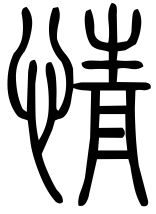
\includegraphics[width=1cm]{Appendices/xin3.png}
({\Large{情}}), & \textit{dzieṅ} ``emotion'' \\
%G:
%SSF: PIF:
人之陰气有欲者。 & ``the yīn-vital energy of man,
the kind which contains desires.'' \\
从心,  & It has {\Large{心}} {\textit{sim}} ``heart'' as a semantic constituent. \\
青聲。 & {\Large{青}} \textit{tsheṅ} 
%(GSR 812c': 
``green, blue, ..''
%) 
is the phonetic constituent.
\end{tabular}

%G As in the case of xīn 心, Xǔ Shèn's gloss is explicitly anthropocentric. He chooses to comment on a rather late psychological use of the word qíng 情 which was current and even dominant in his own time. The graph 情 with the heart radical must indeed be analysed as a Hàn dynasty cultural product. The older uses of the word written by qíng 情 in traditional editions and the rarity of even absence of psychological meaning of qíng 情 discussed and perhaps overstated in A.C. Graham (1967) is thus irrelevant to the origin of the graph. The structure of Chinese graphs must always be discussed as relating to the time of the origin of that graph. The history of characters must be written on the basis of excavated rather than traditionally transmitted texts.
%    The reason why Xǔ Shèn focusses on the psychological meaning rather than the metaphysical ``true nature, essence", is the natural link of the meaning ``emotion'' to the heart radical.
%The graph 情 with the radical to the left of the phonetic is epigraphically unattested Hé Línyí
%何琳儀 1998 dictionary. The word qíng 情 is standardly written with various forms that corre- spond to the phonetic 青. One cannot, in this case, exclude the possibility that the character with

%47 For another instructive case of the use of 自 as a phonetic consider: huì 詯 膽气滿聲。在人上。从言自聲。讀若反目相‰。(荒內切), 自 [疾二切] is phonetic in 詯 [荒內切]!




%its heart radical on the left was indeed invented at the late stage when the word did have its psychological meaning. For example, in Gu\%diàn 郭店 and Shuìhǔdì 睡虎地 manuscripts the character is frequent and apparently never written with the xīn 心 radical and – incidentally – the word xìng 性 is regularly written with the eye radical below 生 rather than the heart radical when it is written with any radical at all.
%    The ``Aristotelian'' genus under which both qíng 情 and xìng 性 are subsumed by Xǔ Shèn is qì 氣 ``vital energy / dynamic force". Both are forms of ``vital energy'' in Xǔ Shèn's cosmological scheme of things. Xǔ Shèn uses the dynamic metaphysical concept of qì 氣 to gloss heart- terminology. This is significant in that he links the realm of the psychological to its physiological/ metaphysical base in his correlative pattern of vital energies.
%    The definition in terms of yīn 陰 precedes the definition in terms of yáng 陽, just as in idiomatic classical Chinese the word order is always yīn yáng 陰陽, never yáng yīn 陽陰. The order of Xǔ Shèn's lexical entries here – as often elsewhere – seems to be determined by word order in classical Chinese. The text of the dictionary is expected to be read consecutively. We shall see more cases of this kind below.
%    Having indicated the genus to which qíng 情 belongs, Xǔ Shèn goes on to specify what kind of yīn 陰-vital energy qíng 情 refers to. However, unlike the case of 媒 謀也謀合二姓 (Shuōwén 12B 443 015)(see above p. 35 under G), Xǔ Shèn does not begin with a full gloss ending in y\% 也. Instead, he appends to his gloss what to the western reader looks like a postposed relative clause. Since there is a y\% 也 at the end of the following strictly parallel entry, one might suspect stylistic carelessness. But our translation tries to take the text seriously, as it stands.
%    Note that yù 欲 ``desire", a manifestly psychological concept, as noted in the introduction, does not here have the heart radical. For the addition of the heart radical see Páng Pǔ 龐樸 (2004).

PIF  qīng 青 (GSR 812c': ``green, blue, ..'') [倉經切; LH {\sil{tsheŋ}}, OCM tshêŋ ] phonetic in qíng
情 [疾盈切; LH {\sil{dzieŋ}}, OCM {\sil{dzeŋ}}]
%PR Many examples show that ts-, tsh- and dz- often freely interchange in phonetic series. This means that phonetic series cannot be used as arguments to reconstruct distinctions between initials like ts-, tsh- and dz-. More generally, phonetic series cannot be used to reconstruct any initials that can be documented to interchange freely in phonetic series.
%    Similarly, many examples show that Old Chinese -êŋ and Old Chinese -eng, though presumably different in pronunciation, interchange freely in phonetic series. This means that phonetic series cannot be used as arguments to reconstruct one of these as opposed to the other. More generally, phonetic series cannot be used to reconstruct any finals that can be documented to interchange frequently in phonetic series.

\subsection{性}

%4. SW 10B. 408: 004; DXB 217 (10B 10a); GL vol 11: 4651b; Duàn 502 (10B 24a); TKJ 1439; Ozaki vol. 5: 995.

\begin{tabular}{ll}
%HG: ə 
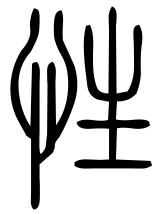
\includegraphics[width=1cm]{Appendices/xin4.png}
({\Large{性}}),	&
\textit{sieṅH} ``inborn nature'' \\
%G: 
人之陽气	& ``the vital yáng-energy of man". \\
%IQ: 
性善者也。 & It is (as in) ``nature is good". \\
%SSF: 
从心, & It has {\Large{心}} {\textit{sim}} ``heart'' as a semantic constituent, \\
%PIF: 
生聲。 & {\Large{生}}  \textit{ṣaeṅ} 
%(GSR 812a: 
``be born, ..''
%) 
is the phonetic constituent.
\end{tabular}

%HG The word xìng 性 was regularly written as sh*ng 生 in pre-Hàn time, and by certain scribes with the eye radical mù 目 below 生. The case of xìng demonstrates the importance of paying attention to the time of invention of characters when discussing their structure.
%G All sorts of things have xìng 性 ``natural endowments", and indeed the sage is known for understanding the xìng 性 of things in general (TLS: Guan, 11). We need to ask why Xǔ Shèn again chooses the anthropocentric perspective on the meaning of the word. Whereas the meaning ``emotion'' may be construed as limited to man, that of ``inborn nature'' applies to living creatures and even to things generally. The presence of the heart radical might be taken to be linked to the fact that xìng 性 is prototypically ascribed to animate creatures, for which in turn humans are the representative example. Also, having provided an explicitly anthropocentric gloss for qíng 情, it was natural to provide a similar gloss for xìng 性.
%IQ   Xǔ Shèn is not making or even agreeing with any claim that nature is good. He merely mentions a current phrase to illustrate the meaning he has attributed to his lexical entry. The modern analytic distinction between use and mention is entirely relevant to an understanding of his text: the phrase 性善 is mentioned not used.
%    The rhythmic parallelism with the preceding lexical entry hides a completely different logical structure. For what Xǔ Shèn provides here is an illustration of the use of the word rather than an elaboration on a semantic nuance. This is a rhetorical device which has a long tradition in classical Chinese literature before Xǔ Shèn's time: superficial parallelism embellishes underlying contrast.
%PIF  The graph 生 is often taken to be not only phonetic but also semantic in function. As we saw in the problematic case of xī 息 above, Xǔ Shèn was prepared to acknowledge the semantic significance of phonetic constituents using the formula 从X, X亦聲. The present example, on the other hand, demonstrates how Xǔ Shèn often fails to acknowledge the manifest semantic relevance of phonetic constituents in his analysis. The formula X聲 is often used in cases where X is also a semantic constituent, and where 从X is omitted. This is what happens in the present instance. One is forced to concede that Xǔ Shèn's formula 从X, X亦聲 could always be abbreviated to 从X, so that the formula 亦聲 must always be regarded as optional. It often remains unclear what motivated Xǔ Shèn's choice of 从X versus X聲 in his analysis. When there is dual function it appears that Xǔ Shèn feels free to specify one or the other, or indeed both functions.

Sh*ng 生 [所庚切; LH {\sil{srɐŋ}}, OCM {\sil{srêŋ}}] phonetic in xìng 性 [息正切; LH {\sil{sieŋᶜ}}, OCM {\sil{seŋh}}]

%PR   Note the contrast in vowel quality as well as in tone. Note also the contrast in the initials.

\subsection{志}
%5. SW 10B 408: 005; DXB 217 (10B 10a); GL vol 11: 4652b; Duàn 502 (10B 24b); TKJ 1439; Ozaki vol. 5: 996, see
%variants in WGY: 447.

\begin{tabular}{ll}
%HG: ¢ 
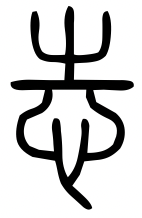
\includegraphics[width=1cm]{Appendices/xin5.png}
({\Large{志}}),      &  \textit{ciH} ``aim/ aspiration'' \\
%G: 
意也。      & is `purpose'. 
%[[is `(a kind of) purpose (scil. concerning one's main orientation or aspiration in life')'.]] 
\\
%SSF: 
从心,      &  It has {\Large{心}} {\textit{sim}} ``heart'' as a semantic constituent, \\
%PIF:  
之聲。      & {\Large{之}} \textit{ci} 
%(GSR 962a: 
``go to, ..''
%) 
is the phonetic constituent.
\end{tabular}

%G Xǔ Shèn defines the species `aspiration' in terms of its genus `idea; purpose'. We indicate this strategy of lexical explanation in our explanatory paraphrase (EP). Wherever possible, we try to make explicit the specificity of the species as opposed to the genus, even when Xǔ Shèn leaves this  to  be  implicitly  understood. We  shall  see  that  also  zh+  䮞 (n°  7  below)  and  tài  態 (n°  130 below) are glossed by the more general 意也 is `purpose'.
%PIF Xǔ Shèn insists on the 之 in his seal script version of the head graph as a phonetic, and this in spite of the fact that he had 士 in the corresponding lìshū 隸書 graph. On the other hand, he does write the seal version of the phonetic by writing its convenient lìshū form: his concern here is with graphemes and not with epigraphic detail.
%    The phonetic zhī 之 may in fact have been chosen for semantic reasons, an aim being something one moves towards, `goes for'. As we have seen already Xǔ Shèn's addition of the formula X亦聲 is less than systematic and often absent where it would seem patently appropriate.
Zhī 之 [止而切; LH {\sil{tshə}}, OCM {\sil{tə}}] phonetic in zhì 志 [職吏切; LH {\sil{tshəᶜ}}, OCM {\sil{təh}}]
%PR   Note the tonal difference.

\subsection{意}

%6. SW 10B 408: 006; DXB 217 (10B 10a); GL vol 11: 4653b; Duàn 502 (10B 24b); TKJ 1439; Ozaki vol. 5: 997, see
%variants in WGY: 447.

\begin{tabular}{ll}
%HG: p 

\includegraphics[width=1cm]{Appendices/xin6.png}
({\Large{意}}), & \textit{qiH}  ``purpose'' \\
%G: 
志也。 & is `aspiration'. %[[is `(like) aspiration (scil. but without reference to higher aims in life)'.]] 
\\
%SN: 
从[read 以]心察言 & Taking one's mind as point of departure one \\
而知意也。 & investigates words and comes to understand ideas/ purposes. \\
%SSF1: 
从心, & It has {\Large{心}} {\textit{sim}} ``heart'' as a semantic constituent, \\
%SSF2: 
从音。& it (also) has {\Large{音}}
\textit{qim} ``sound'' as a semantic constituent.
\end{tabular}

I DON'T THINK THEY HANDLE THIS ONE CORRECTLY.
\footnote{WIKTIONARY: Modern form is a compound of 音 and 心 (“heart”). However, the top component is etymologically unrelated to 音. According to Lin (1920),  (a compound of 言 and 中) found in bronze inscriptions is the same character as 意 (yì). Lin, Yiguang (林義光) (1920). 《文源》. Republished by 中西書局, 2012.}


%G  The terms yì 意 and zhì 志 are used as glosses for each other in the pattern known as hùzhù 互注 or hùxùn 互訓 ``mutual glossing". Such inter-defined terms are many in Shuōwén: Féng Zhēng 馮蒸 1995 lists 354 cases, and adds an important list of 75 more which are created by Duàn's
%emendations of the text. When Xǔ Shèn defines zhì 志 by its hypernym, he adds no illustrative example to make his point clear. On the other hand, when he now employs the word zhì 志 in a strikingly different meaning that has nothing to do with aspirations, but with intended meanings, he adds an elaborate explanation.
%    Duàn rewrites this line as: 意 志也。从心音。察言而知意也。In so doing Duàn surrepti- tiously decides at this point not to rewrite the Dà Xú b\%n but in this case to rewrite the Xi(o Xú b\%n which reads: 意 志也。察言而知意也。從心音聲。
%This Xi(o Xú b\%n text is remarkable in that it declares yīn 音 which has a final nasal to be
%phonetic in yì 意 which has no final nasal. If we were to follow Xi(o Xú b\%n we would have to diagnose a f*i sh*ng 非聲 ``wrong phonetic". See below Shuōwén 10B 408 034 for a listing of declared f*i sh*ng.
%Several inevitably pedantic points need to be made on Duàn's philological procedure here:
%1. Duàn should have advised his readers of the divergence between Dà Xú b\%n and Xi(o Xú b\%n and his choice to base himself primarily on Xi(o Xú b\%n with respect to the postposed gloss, and on Dà Xǔ b\%n with respect to the graphological analysis. (His tacit manipulation of the text is not philologically acceptable by any any standards of Q(ng or modern times.)
%2. Duàn should have advised his readers that he rewrote the Xi(o Xú b\%n's version to say the exact opposite of what it does say. For the Xi(o Xú b\%n regards yīn 音 as phonetic and Duàn declares it to be a semantic constituent.
%3. Duàn should have explained why he changed the standard formula 从心从音 of Dà Xú b\%n to the alternative formula 从心音.
%SN Having expressed our reluctance to rewrite our text before we interpret it, we nonetheless venture to consider a possible emendation for the first character in this line. The received text has the abbreviated variant cóng 从 (Shuōwén gloss: 相聽也) which is largely limited to the technical formula designating a component a semantic constituent. This is not what the character can possibly mean in the present context. We note that the use of the abbreviated cóng 从 as a technical term in our received text is well established only for the Sòng b\%n and that, surprisingly, the fragmentary much earlier and much more reliable Táng dynasty manuscript evidence provides no manuscript support for this Sòng dynasty convention. In the Táng manuscripts the graph 从"have as a semantic constituent'' is always hand-written as 從. In the present case we submit that the use of the simplified cóng in the Sòng edition may conceivably be a mechanical error by a careless scribe who did not understand the important distinction between the technical cóng and the current cóng. Thus one might consider rewriting 从心 as 從心. Another alternative, suggested by Wáng Yún 王筠 (1784-1854) (句讀), is to declare the simplified cóng 从 a plain graphic mistake for y+ 以 which would make even smoother sense but which would assume that someone miswrote the complex 從 first rewritten as simplified 从, since there is no graphic similarity between 從 and 以.
%    The introduction of the technical term simplified 从 as distinct from the verb 從 ``to follow'' remains a crucial development, no matter whether it was made by Xǔ Shèn himself or whether it
%was a creative and congenial innovation by the editors of the DXB. One must remember that the characters 从 and 從 are separate entries in Shuōwén, and that the meaning ``follow'' is attached to the complex cóng 從 (Shuōwén: cóng 從 隨行也) and not to the simplified cóng 从 which is linked to listening/obeying (Shuōwén: cóng 从 相聽也). Xǔ Shèn defines bìng 䮒 as 相從也 and not as 相从也. The gloss 隨從也 recurs twice in Shuōwén (娽 (12B 10a), 楸 (12B 25b)), always in literal contexts of physically following something.
%    Having provided his generic gloss Xǔ Shèn goes on to an analytic elaboration which dispels any impression that he regarded yì 意 and zhì 志 as synonymous just because the two terms are glossed by each other. Whereas it is the purpose of poetry, as described in the Hàn dynasty preface to the Shījīng, to express one's zhì 志 ``aspirations, ultimate motivations", what we understand in the more general case  where we investigate words  are yì 意 ``meanings'' rather than zhì  志"aspirations". (Note that in current Shuōwén usage, yì 意 is sometimes used post-nominally so that X 意也 which often means ``has the meaning X", as in wà 聉:無知意也, ``has the meaning `be ignorant'".)
%SSF2 Surprisingly Xǔ Shèn does not assign any phonetic constituent. This is not uncommon elsewhere, even when modern historical reconstruction might suggest a phonetic role for a constituent.

PR	One notes that the nasal final in yīn 音 prevents it from serving as the phonetic constituent in
yì 意 [於記切; LH {\sil{ʔɨᶜ}}, OCM {\sil{ʔəkh}}]. It appears that Xǔ Shèn never breaks this rule.

\subsection{}

%7. SW 10B 408: 007; DXB 217 (10B 10a); GL vol 11: 4654b; Duàn 502 (10B 25a); TKJ 1439; Ozaki vol. 5: 997.

\begin{tabular}{ll}
%HG: 

\includegraphics[width=1cm]{Appendices/xin7.png} ({\Large{恉}}), & zhǐ, ``main meaning" \\
%G:  
意也。 & is `idea'. 
%[[is `(a kind of) idea (scil. the main idea contained in a text)'.]] 
\\
%SSF:  
从心, & It has {\Large{心}} {\textit{sim}} ``heart'' as a semantic constituent, \\
%PIF: 
旨聲。 &  {\Large{旨}} \textit{ciyX} 
%(GSR 552a: 
``basic idea, ..''
%) 
is the phonetic constituent.
\end{tabular}

%HG The standard way of writing this word in Warring States times as well as in Hàn times is 旨. The phonetic in this graph is in fact the standard way of writing the word in question. Xǔ Shèn records in this instance a specialised orthography the general principles of which have been laid out in Páng Pǔ 龐樸 (2004).
%The standard graph zh+ 旨 is glossed as 美也 and is treated as a composite radical: 从甘匕聲
%(5A 14b).
%G         Xǔ Shèn has the same gloss for zhì 志 `aspiration' and zh+ 䮞 `main meaning'. As indicated before this does not imply that he considered the two words as synonymous. What it does imply is that both concepts belong under the genus `intellectual content, idea' which he denotes by yì 意.



%The only other graph glossed simply as 意也 is: 態:意也。从心从能 ``tài frame of mind is `idea'. It has xīn as a semantic constituent, and it (also) has néng as a semantic constituent."
%PIF      As noted above, the phonetic constituent zh+ 旨 happens to be the most current way of writing the word sometimes written with the heart radical. Declaring this constituent zh+ 旨 to be merely phonetic raises interesting questions: one might be tempted to say that the phonetic is here at the same time a semantic constituent until one realises that in the context of graphological analysis which is relevant to Xǔ Shèn the graphologically pertinent meaning of zh+ 旨 is m\%i 美 `of good taste', a usage well attested in such phrases as zh+ jiǔ 旨酒 ``good wine".
Zh+ 旨 (GSR 552a: ``basic idea, ..'') [職雉切; LH {\sil{tshiᵇ < kiᵇ}}, OCM {\sil{ki)}}] phonetic in zh+ 䮞 [職
雉切; LH {\sil{tshiᵇ < kiᵇ}}, OCM {\sil{ki}})]
%PR   Homophonous phonetic constituent. Moreover it stands to reason that 䮞 and 旨 write one and the same word.

GET READING FROM FANQIE

\subsection{悳}
%8. SW 10B 408: 008; DXB 217 (10B 10b); GL vol 11: 4655b; Duàn 502 (10B 25a); TKJ 1439; Ozaki vol. 5: 998.

\begin{tabular}{ll}
%HG:  
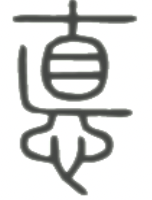
\includegraphics[width=1cm]{Appendices/xin8.png}
({\Large{悳}}), & dé, \\
%G: 
外得於人
 & is what one obtains from others outside, \\
內得於己也。 &  (or) what one obtains for oneself inside. \\
%SSF1: 
从直 & it has {\Large{直}} \textit{ḍiH}
 ``straight'' as a semantic constituent, \\
%SSF2: 
从心, & It (also) has {\Large{心}} {\textit{sim}} ``heart'' as a semantic constituent, \\

\includegraphics[width=10pt]{Appendices/xin8a.png}
{[}從{]}，古文。 & 

\includegraphics[width=15pt]{Appendices/xin8a.png}
is an ancient style graph.
\end{tabular}
%SA: 



%HG In accordance with Warring States palaeographic evidence Xǔ Shèn prefers this graph as the primary way of writing what is currently written as 德. The character 德 itself, which is not unknown from Warring States palaeographic sources, he glosses as 升也 `go up' in order to explain the presence of the marching radical. In this case a graphologically misleading character has come to replace a graphologically transparent character as the standard way of writing the word. (For dé 德 see TKJ: 264, Hé Línyí 1998: 67-68 and for a western account of the epigraphic history of dé see Donald Munro 1969).
%G Xǔ Shèn's philosophical interest seems to interfere with his lexicographic conventions at this point: he omits to tell us what it is that is obtained and seems to assume that the reader knows what it is that constitutes virtue, and goes on to draw a distinction between two sources of this virtue.
%SSF1 Without announcing his emendation, Duàn rewrites the text as 从直心, clearly intending this to be read as 从直、心.
%SSF2 In assigning two semantic constituents to this character, Xǔ Shèn breaks his own convention according to which the first of any two semantic constituents generally is the radical.



HP Zhí 直 [除力切; LH {\sil{drɨk}}, OCM {\sil{drək}}] is not declared phonetic in dé 悳 [多則切; LH {\sil{tək}}, OCM {\sil{tə̂k}}.]
%PR	OCM drək and OCM t*+ k interchange frequently in Xǔ Shèn's phonetic series elsewhere. Thus phonetic series cannot be used to argue for any of these initials.

多 ta
則

GET MC READING FROM FANQIE

\subsection{應}

%9. SW 10B 408: 009; DXB 217 (10B 10b); GL vol 11: 4657/10287; Duàn 502 (10B 25a); TKJ 1440; Ozaki vol. 5: 998.

\begin{tabular}{ll}
%HG: 

\includegraphics[width=1cm]{Appendices/xin9.png}
({\Large{應}}), & qiṅ, \\
%G:  
當也。 & ``should (responding to what is proper)'' is `should fittingly'. \\
%SSF: 
从心,  & It has {\Large{心}} {\textit{sim}} ``heart'' as a semantic constituent, \\
%PIF: 
⿸疒倠聲。 & {\Large{⿸疒倠}} yīng (GSR 890%: ``SW says: eagle [in fact SW says 
`bird')
is the phonetic constituent.
\end{tabular}


%HG The seal graph has the sickness radical instead of the roof radical.
%G	Very often a word is glossed by another word with which it forms a common compound (in this case cf. modern Chinese yīngdāng 應當).
%The realm of obligation is construed as part of psychology.
PIF     yīng ⿸疒倠 = U+24E30(Ext B) (?䧹?) 於陵切; LH {\sil{ʔɨŋ}}, OCM {\sil{ʔəŋ}}] phonetic in [於陵切; LH {\sil{ʔɨŋ}}, OCM {\sil{ʔəŋ}}]

\subsection{慎}

%10. SW 10B 408: 010; DXB 217 (10B 10b); GL vol 11: 4657b; Duàn 502 (10B 25a); TKJ 1440; Ozaki vol. 5: 998.

\begin{tabular}{ll}
%HG:  
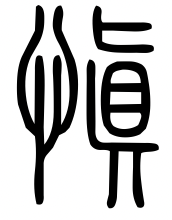
\includegraphics[width=1cm]{Appendices/xin10.png}
({\Large{慎}}) & \textit{jinH}  ``careful" \\
%G: 
謹也。 & is diligent. %[[is `(a way of being) diligent (scil. particularly in paying attention to possible sources of danger)'.]] 
\\
%SSF:  
从心, & It has {\Large{心}} {\textit{sim}} ``heart'' as a semantic constituent,  \\
%PIF: 
真聲。 & {\Large{真}} \textit{cin} 
%(GSR 375a: 
``true, real, ..''
%) 
is the phonetic constituent. \\
%SA: 

\includegraphics[width=10pt]{Appendices/xin10a.png}
{[}昚{]}， 古文。 
& 

\includegraphics[width=15pt]{Appendices/xin10a.png}
is an ancient style graph.
\end{tabular}
%G         Note the collocation j+n shèn 謹慎 which may be taken to motivate the gloss. Note also, in passing,  that  the  equally  psychological  j+n  謹 which  is  so  close  in  meaning  to  shèn  慎 is  not written with the heart radical.
%    The gloss j+n 謹 recurs 6 times in the heart radical alone and it is salutary to remember (see the entries n° 012, 030, 046, 052, 079.)

PIF    zh*n 真 [側鄰切; LH {\sil{tshin}}, OCM {\sil{tin}}] phonetic in shèn 慎 [時刃切; LH {\sil{dzhinᶜ}}, OCM {\sil{dins}}]
%PR Different but regularly interchangeable initials. Different tones. The phonetic rhymes with the character.

\subsection{忠}

%11. SW 10B 408: 011 ; DXB 217 (10B 10b); GL vol 11: 4658b; Duàn 502 (10B 25b); TKJ 1440; Ozaki vol. 5: 999; (Hé
%Línyí: 273)

\begin{tabular}{ll}
HG: ({\Large{忠}}), & \textit{ṭiuwṅ} ``do one's loyal best" \\
G:	敬也。 & is `dedicated'. %[[is `(a way of) being dedicated (scil. by doing one's best for the person one respects)'.]] 
\\
SSF: 从心, & It has {\Large{心}} {\textit{sim}} ``heart'' as a semantic constituent, \\
PIF: 中聲。 & 中 zhǒng (GSR 1007a: ``middle, ..'') is the phonetic constituent.
\end{tabular}

%G   Note that Xǔ Shèn analyses loyal effort in terms of the underlying dedication that motivates it, and of which it is an overt expression.
%SSF According to Xǔ Shèn's analysis the characters zhɨng 忠 and chɨng 忡 (SW 10B 408: 229), though differing in their initials, are taken to have the same phonetic. Moreover their graphonolog- ical analysis is taken to be identical: the placement of the radical is not considered an analytic issue. However, the two graphs write distinct words and pairs like these must be carefully distinguished from allographs pairs like cán 慚/慙 (SW 10B 408: 254).

PIF    中[陟弓切; LH {\sil{truŋ}}, OCM {\sil{truŋ}}] phonetic in 忠 [陟弓切; LH {\sil{druŋ}}, OCM {\sil{druŋ}}]
%PR   Voiced versus unvoiced initials. The phonetic rhymes with the character.

\subsection{愨}

%12. SW 10B 408: 012; DXB 217 (10B 10b); GL vol 11: 4659; Duàn 502 (10B 25b); TKJ 1440; Ozaki vol. 5: 999

\begin{tabular}{ll}
%HG: 
({\Large{愨}}), & què, ``good/earnest" \\
%G:	
謹也。 & is `diligent'. %[[is `(a way of being) diligent (scil. by acting as one should)'.]]
\\
%SSF: 
从心, & It has {\Large{心}} {\textit{sim}} ``heart'' as a semantic constituent, \\
%PIF: 
㱏聲。 & {\Large{㱏}} què (SW: ``strike downwards..'') is the phonetic constituent.
\end{tabular}

%G	The type of goodness què 愨 is analysed in terms of moral diligence.
PIF     㱏[苦角切; LH {\sil{khck}}, OCM {\sil{khrôk}}] phonetic in 愨 [苦角切; LH {\sil{khck}}, OCM {\sil{khrôk}}]
%PR	Phonetic not independently attested as a word in the literature as far as we can see, except in
%Shuōwén itself.


\subsection{⫬}

%13. SW 10B 408: 013; DXB 217 (10B 10b); GL vol 11: 4659b; Duàn 502 (10B 25b); TKJ 1441; Ozaki vol. 5: 1000.

\begin{tabular}{ll}
%HG:	
(⫬), & mi\&o, \\
%G:	
美也。 & is `beautiful/ wonderful'. \\
%SSF: 
从心, & It has {\Large{心}} {\textit{sim}} ``heart'' as a semantic constituent, \\
%PIF: 
焦聲。 &	{\Large{焦}} mào (SW: ``...appearance..'') is the phonetic constituent.
\end{tabular}

PIF     焦 [莫教切;  MC  mauC  =  LH  mauC,  OCM mrâu(k)h]  (see  皃)  phonetic  in  ⫬ [莫角切; MC måk = LH {\sil{mck}}, OCM *{\sil{mrâuk}}]

